\section{Layer 1: Identity and Zero-Trust}

\subsection{Nexa-DID: W3C-Compatible Decentralized Identifiers}

Nexa-net implements a W3C DID Core~\cite{w3c_did_2022}-compatible identifier system called Nexa-DID. The identifier format follows the standard three-part structure:

\begin{equation}
\texttt{did:nexa:<identifier>} \quad \text{where} \quad \text{identifier} = \text{hex}(\text{SHA-256}(\text{pk}_{\text{Ed25519}})[0:40])
\end{equation}

The identifier is derived deterministically from the agent's Ed25519 public key using SHA-256 truncated to the first 40 bytes, encoded in hexadecimal. This approach ensures that: (1) the DID is globally unique, as different Ed25519 keys produce different hashes with negligible collision probability; (2) the DID is self-certifying, as anyone who knows the public key can verify the DID derivation; and (3) the DID is permanent, as the identifier does not change unless the agent's fundamental identity key is rotated.

The DID generation algorithm benchmarks at 18.71\textmu s for Ed25519 keypair generation and 9.75\textit{ns} for DID string parsing (validation of the \texttt{did:nexa:<hex>} format), making identity operations negligible overhead compared to the 31\textmu s semantic routing latency.

\subsection{DID Document Structure}

Each Nexa-DID resolves to a DID Document conforming to the W3C specification. The document includes:

\begin{itemize}
  \item \texttt{verificationMethod}: An Ed25519 public key entry with type \texttt{Ed25519VerificationKey2020}, used for message signing and authentication.
  \item \texttt{keyAgreement}: An X25519 public key entry with type \texttt{X25519KeyAgreementKey2020}, used for Diffie-Hellman key exchange during mTLS session establishment.
  \item \texttt{authentication}: A reference to the Ed25519 verification method, indicating that the DID controller can authenticate using this key.
  \item \texttt{service}: A \texttt{NexaProxyEndpoint} entry pointing to the agent's proxy HTTP endpoint (e.g., \texttt{https://proxy.nexa.net:7070}).
\end{itemize}

The DID Document is stored locally in the agent's \texttt{MemoryStore} and published to the Kademlia DHT for network-wide resolution. The \texttt{DIDResolver} module implements a two-phase resolution strategy: first check the local cache (117\textit{ns} lookup), then query the DHT if the DID is unknown. Resolution results are cached with TTL-based expiration.

\subsection{Ed25519/X25519 Key Management with Zeroize}

Key management follows a rigorous security design using the ed25519-dalek~\cite{ed25519dalek2022} and x25519-dalek Rust crates. The \texttt{IdentityKeys} structure holds three key pairs:

\begin{enumerate}
  \item \textbf{Signing key} (Ed25519): Used for DID authentication, MicroReceipt payer/payee signatures, and VC credential signing.
  \item \textbf{Key agreement key} (X25519): Used for mTLS Diffie-Hellman exchange to establish shared secrets.
  \item \textbf{Identity key} (Ed25519): The master identity key from which the DID identifier is derived, used only for DID Document updates and key rotation authorization.
\end{enumerate}

All private key material is protected by the \texttt{zeroize} crate~\cite{zeroize2022}, which ensures that private key bytes are securely cleared from memory when the key object is dropped. The \texttt{ZeroizeOnDrop} trait is implemented for all key types, guaranteeing that no private key material remains in heap or stack memory after the object's lifetime ends. This mitigates cold-boot attacks and memory-scanning exploits.

Full identity key set generation benchmarks at 34.98\textmu s (covering Ed25519 signing key, X25519 key agreement key, and the master identity key). Individual signing operations measure 34.68\textmu s (Ed25519 sign) and 38.54\textmu s (Ed25519 verify), consistent with the ed25519-dalek library's reference benchmarks.

\subsection{Verifiable Credentials: Issuance and Verification}

Verifiable Credentials~\cite{w3c_vc_2022} provide the trust layer for capability attestation. A VC in Nexa-net follows this structure:

\begin{itemize}
  \item \texttt{issuer}: The DID of the Trust Anchor that issued the credential.
  \item \texttt{subject}: The DID of the agent whose capability is being attested.
  \item \texttt{credentialSubject.capability}: The capability claims (e.g., accuracy score, average latency, availability).
  \item \texttt{proof}: An Ed25519 signature over the credential content, created by the issuer.
\end{itemize}

The \texttt{VerifiableCredential} module implements issuance (VC creation + Ed25519 signing by the Trust Anchor) and verification (signature check + trust chain validation + expiration check). Property-based tests with proptest~\cite{proptest2019} generate random credential content and verify that: (1) a properly issued VC always passes verification; (2) a tampered VC always fails verification; (3) an expired VC always fails verification; (4) a VC issued by an untrusted anchor always fails verification. These properties are validated across 1000 random iterations.

\subsection{mTLS Mutual Authentication}

Mutual TLS (mTLS) provides bidirectional authentication for proxy-to-proxy communication. In Nexa-net's mTLS design, each proxy generates a short-lived X.509 certificate derived from its Ed25519 signing key, with the DID identifier embedded in the certificate's Subject Alternative Name (SAN) URI field. The certificate signing request (CSR) is self-signed---there is no external certificate authority, as the DID Document serves as the trust anchor.

The mTLS handshake proceeds as follows: (1) Proxy A presents its DID-derived certificate; (2) Proxy B resolves DID A via the DHT, retrieves DID Document A, and verifies that the certificate's public key matches the DID Document's \texttt{authentication} verification method; (3) Proxy B presents its own DID-derived certificate; (4) Proxy A performs the same resolution and verification for DID B; (5) Both proxies derive a shared secret via X25519 key agreement and establish an encrypted TLS 1.3 session.

\textbf{Implementation status:} The mTLS module defines the handshake protocol, certificate generation logic, and DID-verification integration, but the actual TLS session establishment is a design placeholder awaiting integration with the Rust \texttt{rustls} library for production use.

\subsection{Trust Anchor}

The Trust Anchor is the root of the VC trust chain. In Nexa-net, multiple Trust Anchors can operate simultaneously, each identified by its own DID. A Trust Anchor's DID Document includes a \texttt{nexa:trustAnchor} service endpoint that accepts VC issuance requests.

The trust verification algorithm checks: (1) the VC issuer's DID resolves to a valid DID Document; (2) the issuer is recognized as a Trust Anchor (listed in the network's anchor registry); (3) the VC's Ed25519 signature is valid against the issuer's verification method; (4) the VC has not expired; and (5) the VC's subject DID matches the agent claiming the capability. If any check fails, the VC is rejected and the agent's capability claims are downgraded to unverified status (quality score defaults to 0.5 instead of the claimed value).

\begin{figure}[t]
\centering
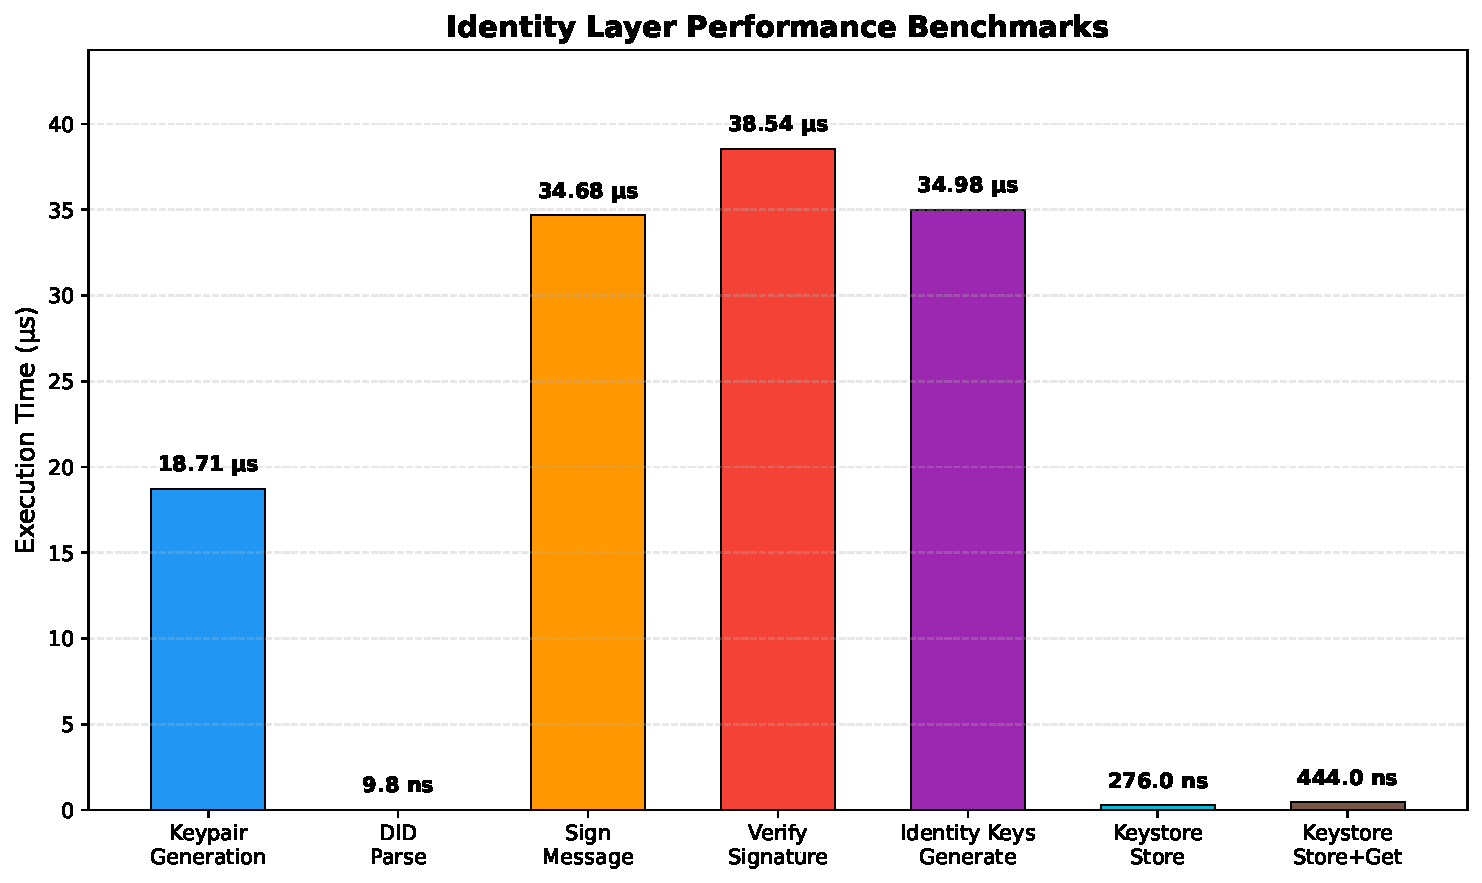
\includegraphics[width=0.85\columnwidth]{figures/identity_bench.pdf}
\caption{Identity layer performance benchmarks. DID parsing is negligible (9.75\textit{ns}); Ed25519 operations are in the 35--39\textmu s range, suitable for receipt verification.}
\label{fig:identity-bench}
\end{figure}